% \subsection{実験概要}
% 提案手法によるより自然な敵対的サンプルが生成可能なのかどうか有効性を検証するため,敵対的サンプルの生成実験を行った.前述の通り,提案手法に示した重要度算出法と離散化手法を組み合わせ,敵対的サンプルを生成する.さらに,得られた敵対的サンプルの具体的な値について,適切か否かの確認を行う.
\subsection{実験条件}
今回の実験は,銀行のローンの審査システムについての機械学習モデルを想定し,誤分類を引き起こす敵対的サンプルの生成を行うことを目的とした.パラメータの設定は従来研究\cite{ballet2019imperceptible}に準拠している.式(5)で示したバランスを $\lambda=8.5$,最大イテレーション数が20000回,ニューラルネットワークの勾配降下法で使用する学習率を $\alpha=0.001$ とする.今回使用する機械学習モデルは,12個の特徴量を入力とし,2つのクラス(承認または拒否)を出力するニューラルネットワークである.このネットワークは,100個のノードを持つ隠れ層が6層にわたって配置された全結合型のモデルである.隠れ層はReLU関数で活性化され,出力層はバイナリクラス分類のためにシグモイド関数が使用されている.これらのモデルを図示したものを下に示す.

\begin{figure}[H]
    \centering
    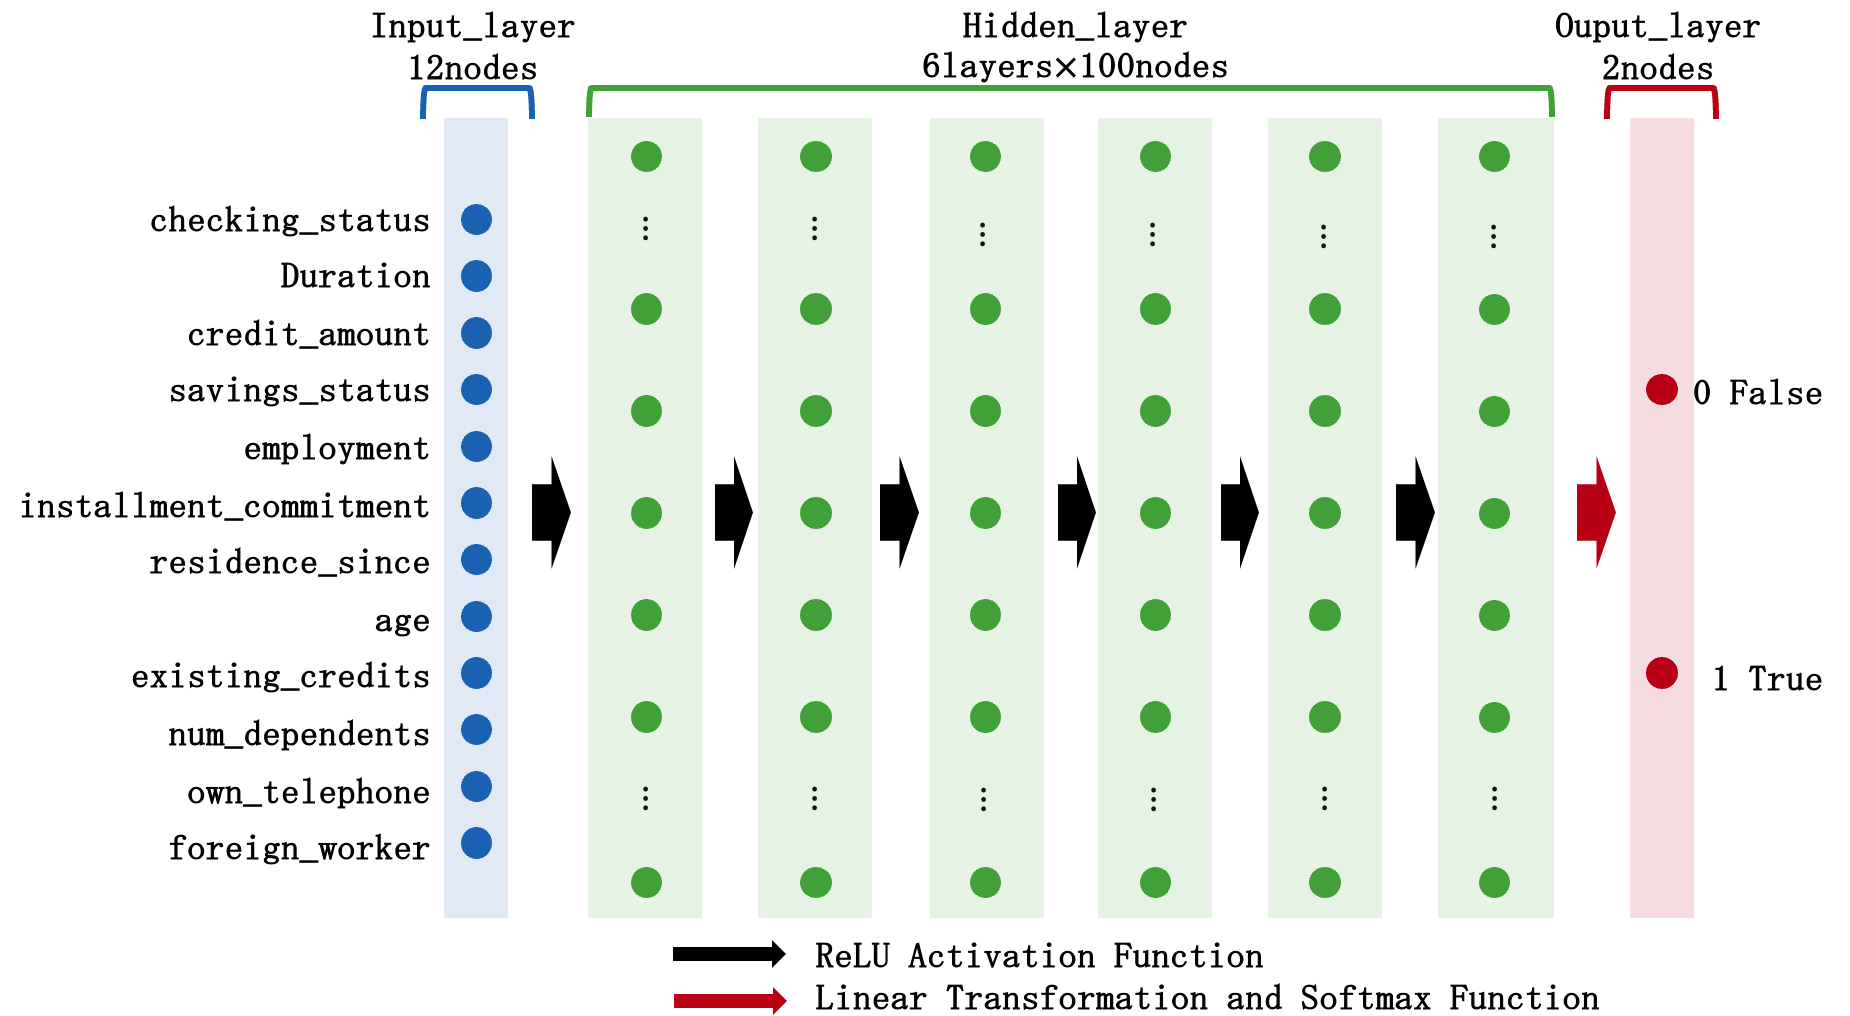
\includegraphics[width=0.8\textwidth]{images/審査モデル.png}
    \caption{銀行のローン審査を行う機械学習モデルの構造}
    \label{fig:adversarial_example}
\end{figure}

また,学習においてBCELoss(Binary Cross Entropy Loss)が損失関数として使用している.モデルが各サンプルに対して予測した確率と実際のラベルとの誤差を計算し,二値分類における誤差を最小化する.最適化アルゴリズムにはAdamを使用し,学習率は $1.0 \times 10^{-4}$ に設定されている.バッチ学習を行い,バッチサイズは $N=100$ となっている.データを小分けにして学習を進め,予測精度はkeras.utils.to\_categoricalを用いてワンホットエンコーディングに変換し,各バッチで予測精度を計算した後,全データで平均を取っている.これによりモデルの分類精度を評価する.

\subsection{使用するデータセット}
これまでに説明した敵対的サンプルの生成手法を検証するため,実験に使用するデータセットについて説明する.

今回使用するデータは,OpenMLで公開されているUCI Machine Learnning RepositoryのGerman Credit Data Setである.\cite{credit-g}このデータセットは,ローンの信用リスクを予測する二値分類問題を扱っており,金融業界での実用的なモデル適用を想定した研究に適している.また,カテゴリカルデータと数値データの両方を含んでおり,敵対的サンプル生成手法の多様な適用可能性を評価するのに適した構造を持っている.このデータセットで使用した特徴量は,以下の通りである.

\begin{table}[H]
    \centering
    \caption{信用情報データセットの特徴量(ドイツマルク建)}
    \begin{tabular}{|l|l|l|}
        \hline
        特徴量名 & 属性 & 種類 \\ \hline
        checking\_status & 既存の当座預金口座のステータス & カテゴリ \\ \hline
        duration & ローン申請期間(月) & 数値 \\ \hline
        credit\_amount & クレジットの金額(申請する与信金額) & 数値 \\ \hline
        savings\_status & 貯蓄口座/債券のステータス & カテゴリ \\ \hline
        employment & 現在の雇用年数 & カテゴリ \\ \hline
        installment\_commitment & 可処分所得に対する分割払いの割合 & 数値 \\ \hline
        residence\_since & X年からの現在の居住地 & 数値 \\ \hline
        age & 年齢 & 数値 \\ \hline
        existing\_credits & この銀行の既存クレジット数 & 数値 \\ \hline
        num\_dependents & 扶養家族数 & 数値 \\ \hline
        own\_telephone & 電話 & カテゴリ \\ \hline
        foreign\_worker & 外国人労働者 & カテゴリ \\ \hline
        target & ローン承認 (true) or ローン却下(false) & カテゴリ \\ \hline
    \end{tabular}
    \label{tab:credit_g_features}
\end{table}

ここで上記の特徴量について追加の説明を行う.checking\_statusは顧客の当座預金口座を4つステータスを示しており,債務がある状態,200マルク以下の少額の預金がある状態,銀行の講座を保有していない状態,200マルク以上の多額の預金がある状態を指している.savings\_statusは貯蓄を4つのステータスで示しており,貯蓄が確認できない状態,貯蓄が100ドイツマルク以下の少額の貯蓄しかない状態,500マルク以下の少額から中程度の貯蓄がある状態,1000マルク以下の中程度の貯蓄がある状態,それ以上の高額な貯蓄がある状態を示している.また,表1で種類がカテゴリである特徴量についてはダミー変数化し離散値として扱う.また種類が数値である特徴量についても全て離散値であることがわかった.このデータセットは,ローンの信用リスクを予測するためのデータセットであるため,ローンの承認結果を予測する二値分類問題として扱う.

実験では,1000件のデータに対して正解データのバランスを保つようにデータをサンプリングする.取得した600件のデータのうち300件を学習データ,250件をテストデータ,残りを検証データに分割する.
まず,学習データでモデルの学習を行い,その後テストデータによるモデルの評価を行う.次にテストデータからランダムに10件取得し,それらをベースにノイズを加え敵対的サンプルを生成する.生成された敵対的サンプルに対して以下の評価指標を用いて評価を行う.

\subsection{評価指標}
提案手法の有効性の評価として以下の3つの指標を用い比較を行う.

一つ目に敵対的サンプルが元データと異なるクラスに分類されることを評価する成功率という指標である.ここで $\tilde{X}$ は生成された敵対的サンプルが元データと異なるクラスに分類されたサンプルの集合であり,$X$ は生成された敵対的サンプルのベースとなった元データのサンプルの集合である.以下の式(9)に示す.
\autoequation{成功率 = \cfrac{|\tilde{X}|}{|X|}}
この指標が大きいほど敵対的サンプルが元データと異なるクラスに分類されることが多いことを示す.

二つ目に敵対的サンプル生成前のサンプルと生成後のサンプル間の距離を評価する指標である.まず,先ほどの敵対的サンプルとそのベースとなった元データのサンプルの集合について以下のように定義する.
\autoequation{X = [\bm{x}_1, \bm{x}_2, \cdots, \bm{x}_N ]}
以上をふまえ,以下の式(10)を平均距離として評価する.
\autoequation{平均距離 = \cfrac{1}{N} \sum^{N}_{i=1} \sqrt{\sum^{d}_{j=1}(x_{i, j}-\tilde{x}_{i, j})^2}}

これは,敵対的サンプルとその元になったデータの差分を求めている.これは敵対的サンプルを生成する過程で加えられたノイズの大きさを表しており,この指標が小さいほどノイズが小さく,元データに近いサンプルが生成されていることを示す.

三つ目に先ほどの平均距離に対して各特徴量の重要度で重み付けした指標である.これを重み距離と呼び,式(11)に示す.
\autoequation{重み距離 =  \cfrac{1}{N} \sum^{N}_{i=1} \sqrt{\sum^{d}_{j=1}( | x_{i, j}-\tilde{x}_{i, j}| \cdot v_j )^2}}
ここでは先ほどの平均距離で計算していた敵対的サンプルとその元になったデータの距離に対して,式(6)で定義した重要度を $\bm{v_j}$ とし,重み付けを行った距離を求めている.これは,重要度の高い特徴量へノイズを加えることで,目立ちやすく人間が知覚しやすい変更が行われていることを意味してしまう.よって,敵対的サンプルの定義である人間が知覚しずらいノイズであるかどうかを判断するためこの指標を用いる.平均距離同様この値が小さいほどより自然で人間が知覚しずらいノイズを付加したことがわかる.

各指標を組み合わせて使用することで,生成した敵対的サンプルの「有効性」と「自然さ」の両面を総合的に評価することを目指す.

\subsection{実験結果}
実験結果について確認する.上記の評価指標に加えて,各手法における重要度特徴量と生成された敵対的サンプルの具体的な値についても確認する.

\subsubsection{成功率}
成功率について確認する.
\begin{table}[H]
    \centering
    \caption{実験結果:成功率}
    \begin{tabular}{|c|c|c|c|} \hline
        離散化 & 従来手法( $\bm{v}$ ) & 重要度算出( $\bm{v}_{\mathrm{raw}}$ ) & 重要度算出( $\bm{v}_{\mathrm{sqrt}}$ ) \\ \hline
        なし & 1.0 & 1.0 & 1.0 \\ \hline
        離散化(四捨五入) & 1.0 & 1.0 & 1.0 \\ \hline
        離散化(ランダム) & 1.0 & 1.0 & 1.0 \\ \hline
    \end{tabular}
\end{table}
すべての手法で10個の敵対的サンプルの生成ができた.これにより,提案手法による敵対的サンプルの精度の悪化などは発生していないことがわかる.よって,以降の平均距離,重み距離についてこの10個のサンプルを用いて評価を行っていく.

\subsubsection{平均距離}
平均距離について確認する.
\begin{table}[H]
    \centering
    \caption{実験結果:平均距離}
    \begin{tabular}{|c|c|c|c|} \hline
        離散化 & 従来手法( $\bm{v}$ ) & 重要度算出( $\bm{v}_{\mathrm{raw}}$ ) & 重要度算出( $\bm{v}_{\mathrm{sqrt}}$ ) \\ \hline
        なし & 0.377 & 0.260 & 0.173 \\ \hline
        離散化(四捨五入) & 0.399 & 0.264 & 0.163 \\ \hline
        離散化(ランダム) & 0.454 & 0.347 & 0.233 \\ \hline
    \end{tabular}
\end{table}
この結果から,従来手法よりも提案手法は,元データに近い敵対的サンプルを生成できていることがわかる.特に,重要度算出法( $\bm{v}_{\mathrm{sqrt}}$ )を用いた場合,最も小さい平均距離を示しており,元データに対する変更が最小限に抑えられていることが確認できる.離散化手法については四捨五入の方がよりノイズが小さくなっていることがわかる.これは,四捨五入による離散化が元データの特徴をより忠実に保持しているためと考えられる.さらに,重要度算出法( $\bm{v}_{\mathrm{sqrt}}$ )を用いた場合,四捨五入による離散化手法では,この実験で最小の平均距離を示している.これは,提案手法が元データの特徴を捉えつつ,適切なノイズを付加することで,より自然な敵対的サンプルを生成できていることを示している.また,従来手法( $\bm{v}$ )と比較して,提案手法( $\bm{v}_{\mathrm{raw}}$ および $\bm{v}_{\mathrm{sqrt}}$ )は,いずれの離散化手法においても平均距離が小さくなっている.これにより,提案手法が従来手法に比べて,より効果的に敵対的サンプルを生成できることが示されている.

\subsubsection{重み距離}
重み距離について確認する.
\begin{table}[H]
    \centering
    \caption{実験結果:重み距離}
    \begin{tabular}{|c|c|c|c|} \hline
        離散化 & 従来手法( $\bm{v}$ ) & 重要度算出( $\bm{v}_{\mathrm{raw}}$ ) & 重要度算出( $\bm{v}_{\mathrm{sqrt}}$ ) \\ \hline
        なし & 0.043 & 0.060 & 0.173\\ \hline
        離散化(四捨五入) & 0.044 & 0.048 & 0.061 \\ \hline
        離散化(ランダム) & 0.051 & 0.105 & 0.105 \\ \hline
    \end{tabular}
\end{table}
この結果から,提案手法は従来手法よりも良いスコアを出すことができなかった.特に,重要度算出( $\bm{v}_{\mathrm{sqrt}}$ )を用いた場合,重み距離が大きくなっていることが確認できる.これは,重要度算出法( $\bm{v}_{\mathrm{sqrt}}$ )が重要度の高い特徴量の値を小さくしてしまったため,ノイズの発生率を高めてしまったことが考えられる.一方で,重要度算出( $\bm{v}_{\mathrm{raw}}$ )における四捨五入による離散化手法では,従来手法に最も近い距離を示している.これは,四捨五入による離散化が元データの特徴を保持しつつ,適切なノイズを付加することで,重み距離を抑える効果があったと考えられる.また,離散化手法についても興味深い結果が得られた.離散化を行わない場合,提案手法( $\bm{v}_{\mathrm{raw}}$ )および( $\bm{v}_{\mathrm{sqrt}}$ )は従来手法よりも重み距離が大きくなっている.これは,連続値の敵対的サンプルが元データの分布から大きく逸脱しているためと考えられる.一方で,四捨五入による離散化手法を用いることで,重み距離が従来手法に近づいていることが確認できる.さらに,ランダム離散化手法では,提案手法( $\bm{v}_{\mathrm{raw}}$ )および( $\bm{v}_{\mathrm{sqrt}}$ )の重み距離が大きくなっている.これは,ランダム離散化が元データの特徴を保持する効果が低いためと考えられる.以上の結果から,提案手法は従来手法に比べて重み距離の面で劣る部分があるものの,重要度算出( $\bm{v}_{\mathrm{raw}}$ )と四捨五入による離散化手法の組み合わせが最も効果的であることが示された.この組み合わせにより,元データの特徴を保持しつつ,適切な敵対的サンプルを生成することができる.

\subsubsection{特徴量重要度}
従来手法($\bm{v}$),提案手法($\bm{v}_{\mathrm{raw}}$),提案手法($\bm{v}_{\mathrm{sqrt}}$)における特徴量重要度について以下の図に示す.
% 青色が従来手法($\bm{v}$),黄色が提案手法($\bm{v}_{\mathrm{raw}}$),緑色が提案手法($\bm{v}_{\mathrm{sqrt}}$)である.
\begin{figure}[H]
    \centering
    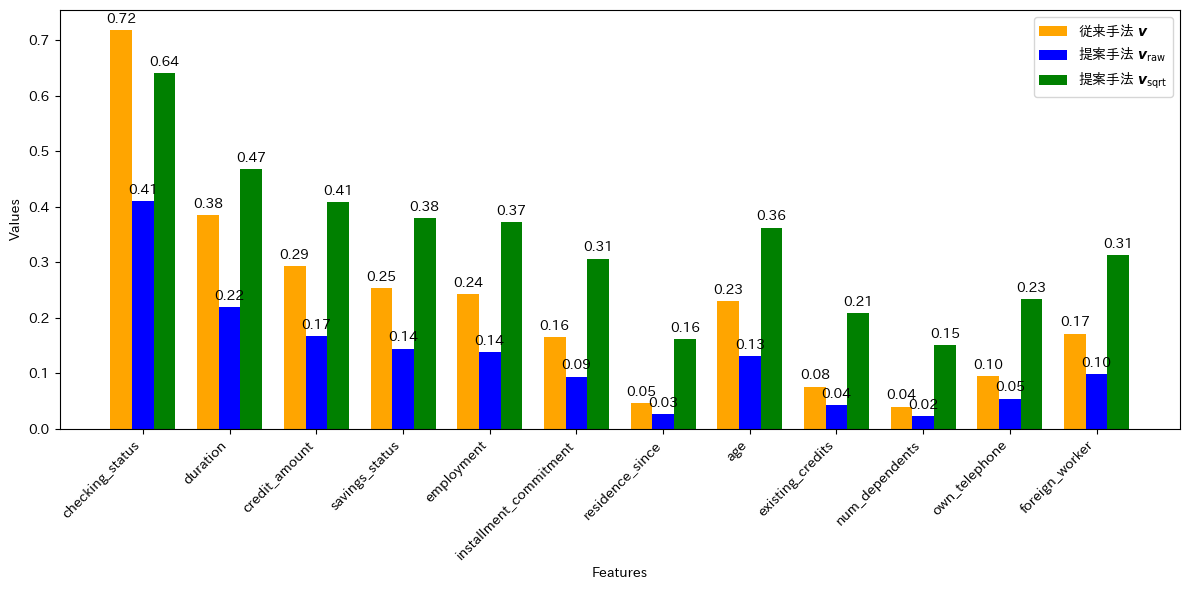
\includegraphics[width=0.8\textwidth]{images/実験_重要度算出の結果.png}
    \caption{各特徴量における重要度}
    \label{fig:adversarial_example}
\end{figure}
重要度について比較すると,従来手法では,checking\_statusに対する重要度が最も高く,次に重要度の高いdurationやcredit\_amountとの差が大きく離れていることがわかる.提案手法ではその差が小さくなっていることが確認できる.また,提案手法( $\bm{v}_{\mathrm{sqrt}}$ )では,特徴量の重要度がより均等になっていることがわかる.これにより,提案手法はより自然な敵対的サンプルを生成できることが示された.

\subsubsection{生成された敵対的サンプルの結果}
最後に,従来手法,提案手法によって生成された敵対的サンプルについて確認する.前述の使用するデータセットで説明したように,10件のサンプリングされたデータが元になっているため,それぞれ敵対的サンプルのベースとなるデータと比較を行う.今回は提案手法の実験の中で最も良い結果を示した重要度算出( $\bm{v}_{\mathrm{sqrt}}$ )における離散化(四捨五入)手法を用いて生成された敵対的サンプルについて比較を行う.

\begin{table}[H]
    \centering
    \caption{元データと敵対的サンプルの比較(id=268)}
    \begin{tabular}{|c|c|c|c|} \hline
        特徴量 & 元データ & 従来手法 & 提案手法 \\ \hline
        checking\_status & 0 & 0.09115 & 0 \\ \hline
        duration & 14 & 8.89098 & 15 \\ \hline
        credit\_amount & 8978 & 7153.84454 & 9169 \\ \hline
        savings\_status & 0 & 0.08376 & 0 \\ \hline
        employment & 4 & 3.94764 & 4 \\ \hline
        installment\_commitment & 1 & 1.07192 & 1 \\ \hline
        residence\_since & 4 & 4.00000 & 2 \\ \hline
        age & 45 & 44.41327 & 45 \\ \hline
        existing\_credits & 1 & 1.00000 & 1 \\ \hline
        num\_dependents & 1 & 1.00000 & 1 \\ \hline
        own\_telephone & 1 & 0.99231 & 1 \\ \hline
        foreign\_worker & 1 & 1.00000 & 1 \\ \hline
    \end{tabular}
\end{table}

全体として,提案手法では離散化により自然な敵対的サンプルになっていることがわかる.また,ノイズの大きさについては,idが268であるデータに注目するとchecking\_statusのノイズの回避が強くなり,durationやcredit\_amountに対してノイズが大きくなっている従来手法に対して,提案手法ではこれらの問題を抑えることができている.これにより,特定の特徴量に対する強いノイズを避ける傾向を抑え,なおかつ他の重要度の高い特徴量へのノイズを小さくすることができている.よって提案手法はより自然な敵対的サンプルを生成できることが示された.
